\documentclass[pdftex]{beamer}
\usepackage[ruled]{algorithm2e}
\usepackage{algorithmic}
%\usetheme{Frankfurt}

% declare the path(s) where your graphic files are
% ../.. is the GeocronDocuments directory
\graphicspath{{../../images/diagrams/}}
\DeclareGraphicsExtensions{.pdf,.png}

\begin{document}

\title[Short Title]{Simulating Disaster Scenarios and Geographically-Correlated Resilient Overlay Networks}
\subtitle{Heuristics for Location-based Routing}
\author[K. Benson and Z. Huang]{Kyle E. Benson and Zhipeng Huang}
\institute[UCI]{
  Department of Computer Science\\
  University of California, Irvine\\
  Irvine, California 92697\\[1ex]
  \texttt{kebenson@uci.edu} and \texttt{zhipengh@uci.edu}
}

% % % % % % % % % % % % % % % % % % % % % % % % % % % % % % % % % % % % % % % % % %

\begin{frame}[plain]
	\titlepage
\end{frame}

% % % % % % % % % % % % % % % % % % % % % % % % % % % % % % % % % % % % % % % % % %

\begin{frame}{Exploiting Location Information}
\begin{columns}
\begin{column}{.5\textwidth}

\begin{itemize}
	\item Contact overlay nodes outside of local region to avoid failures
	\item Choose overlay nodes from diverse regions not previously attempted
	\item Failure likely along path to server or in local area
	\item Choose node outside local	region to avoid overlapping	paths
	\item Choose path avoiding as much of the direct path as possible
	\item Overlay node may use similar route to sensor
\end{itemize}
\end{column}
	
\begin{column}{.5\textwidth}
\begin{figure}
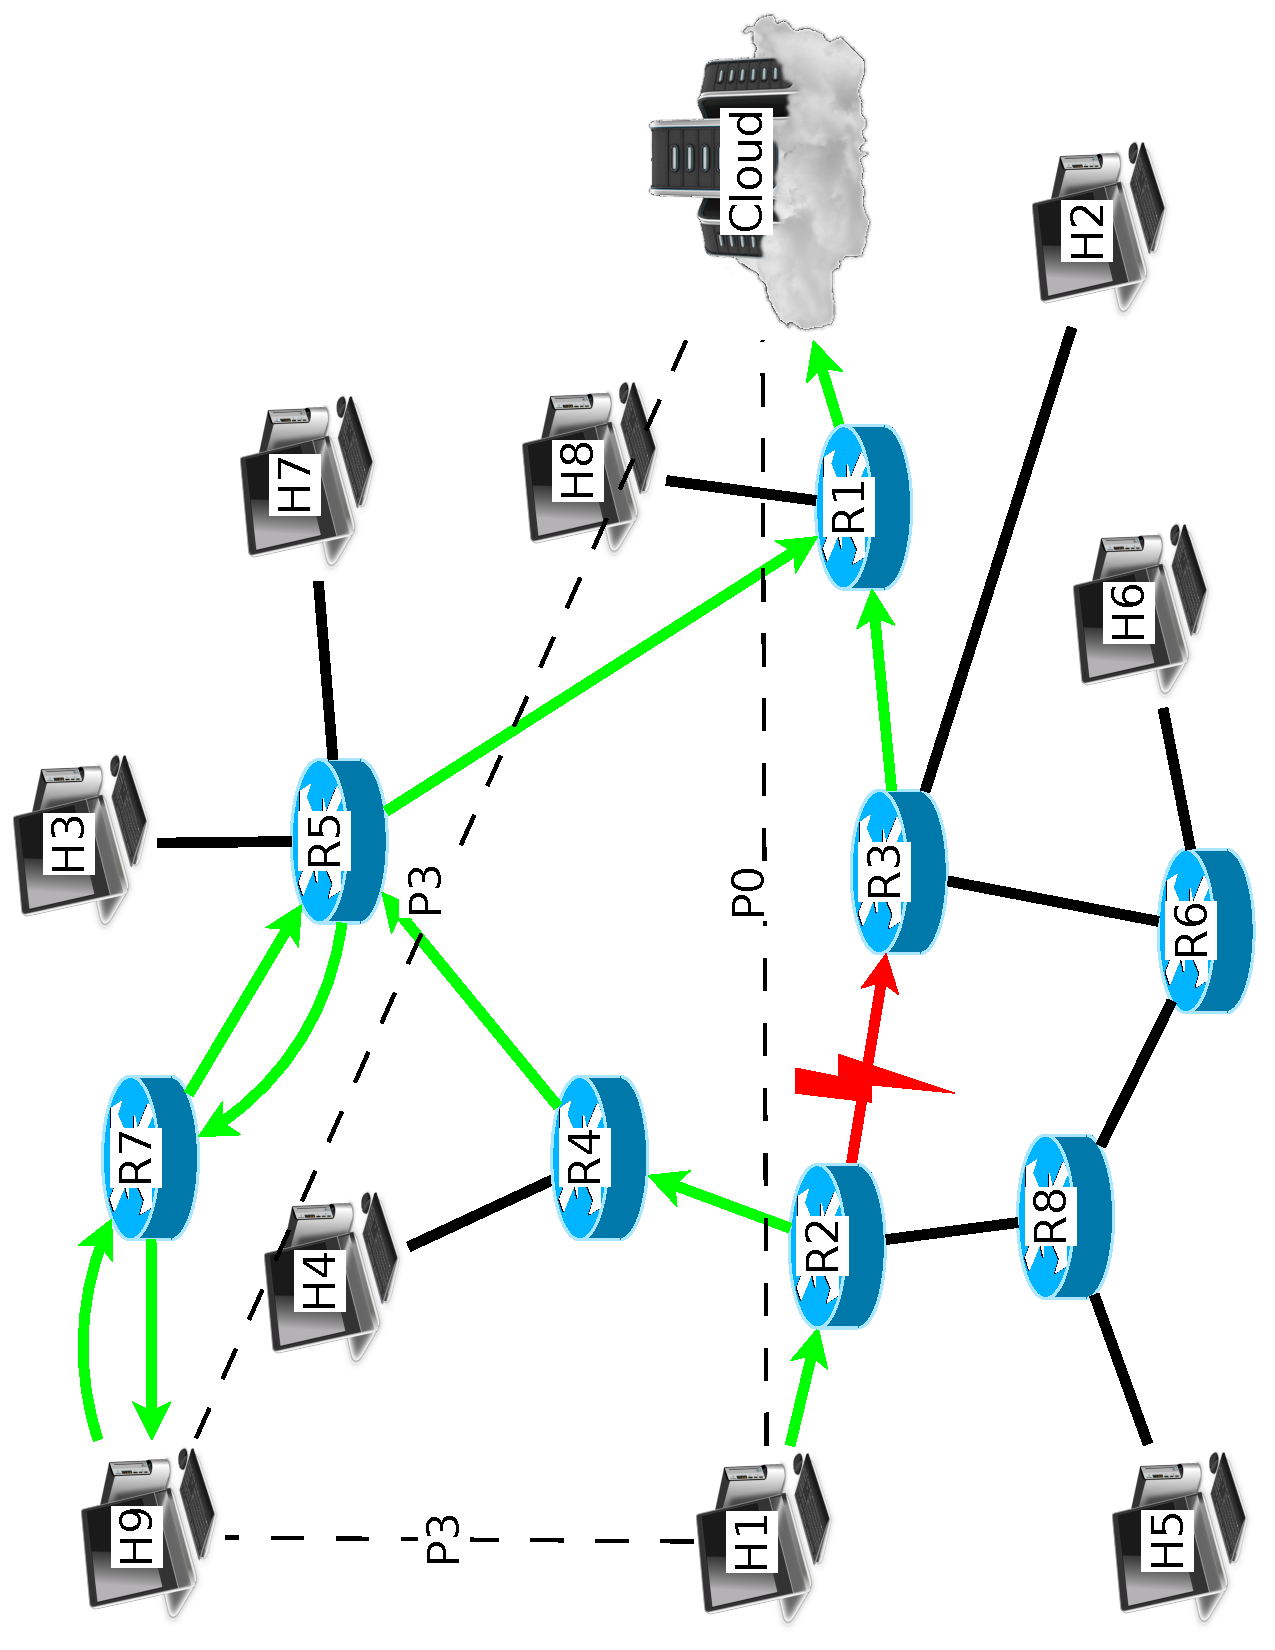
\includegraphics[height=\textwidth,angle=-90]{exploiting_location_information}
\caption{Sensors try to contact nodes outside of the local area and not along the straight-line path to the server.}
\end{figure}
\end{column}

\end{columns}
\end{frame}

% % % % % % % % % % % % % % % % % % % % % % % % % % % % % % % % % % % % % % % % % %

\begin{frame}{Orthogonal Distant Path Heuristic}
\begin{columns}
\begin{column}{.5\textwidth}


% orthogonal algorithm goes here

\end{column}
	
\begin{column}{.5\textwidth}
\begin{figure}
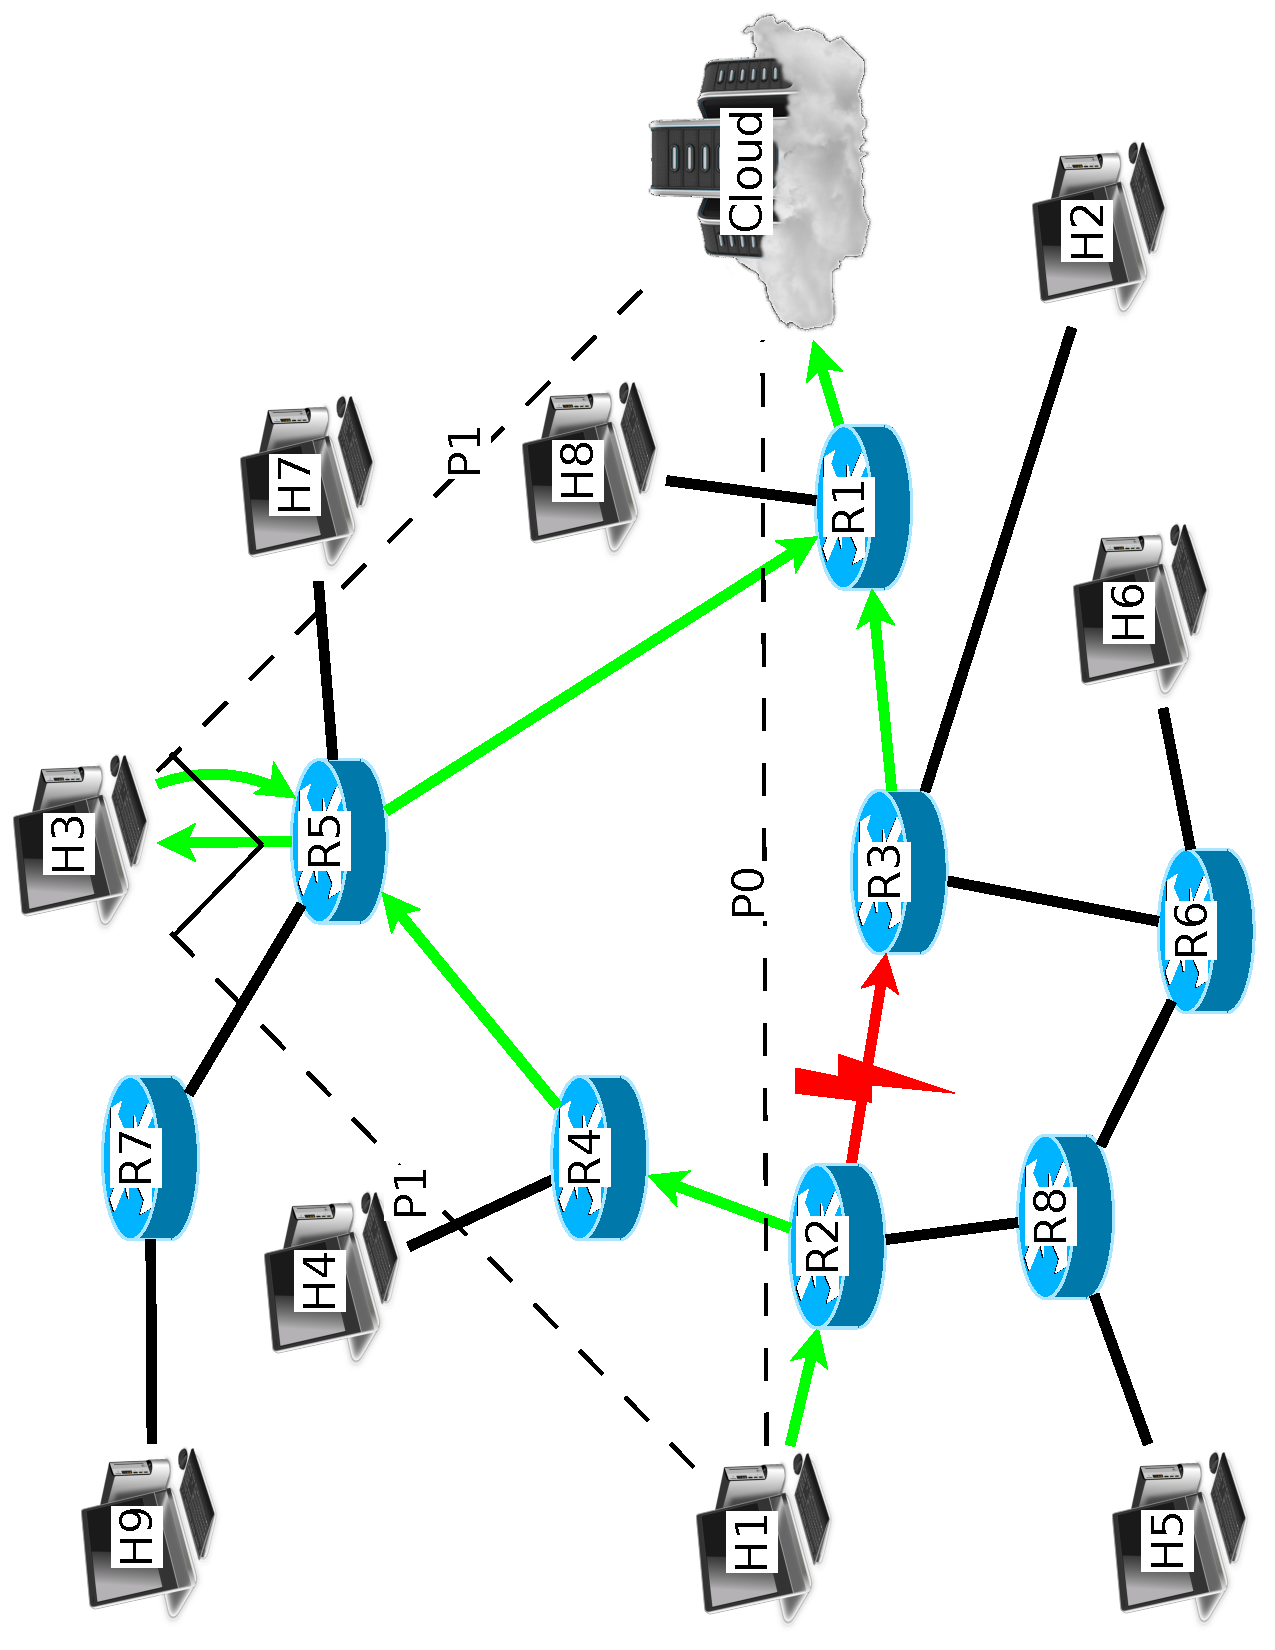
\includegraphics[height=\textwidth,angle=-90]{angular_path}
\caption{The intuition of this heuristic is to avoid the straight path, without diverging from it too much.  It strikes a middle ground by choosing a path at an ideal angle of $45^{\circ}$, which makes the angle at the top orthogonal, hence the name.}
\end{figure}
\end{column}

\end{columns}
\end{frame}

% % % % % % % % % % % % % % % % % % % % % % % % % % % % % % % % % % % % % % % % % %

\begin{frame}{New Region Heuristic}
\begin{columns}
\begin{column}{.5\textwidth}


% newregion algorithm goes here

\end{column}
	
\begin{column}{.5\textwidth}
\begin{figure}
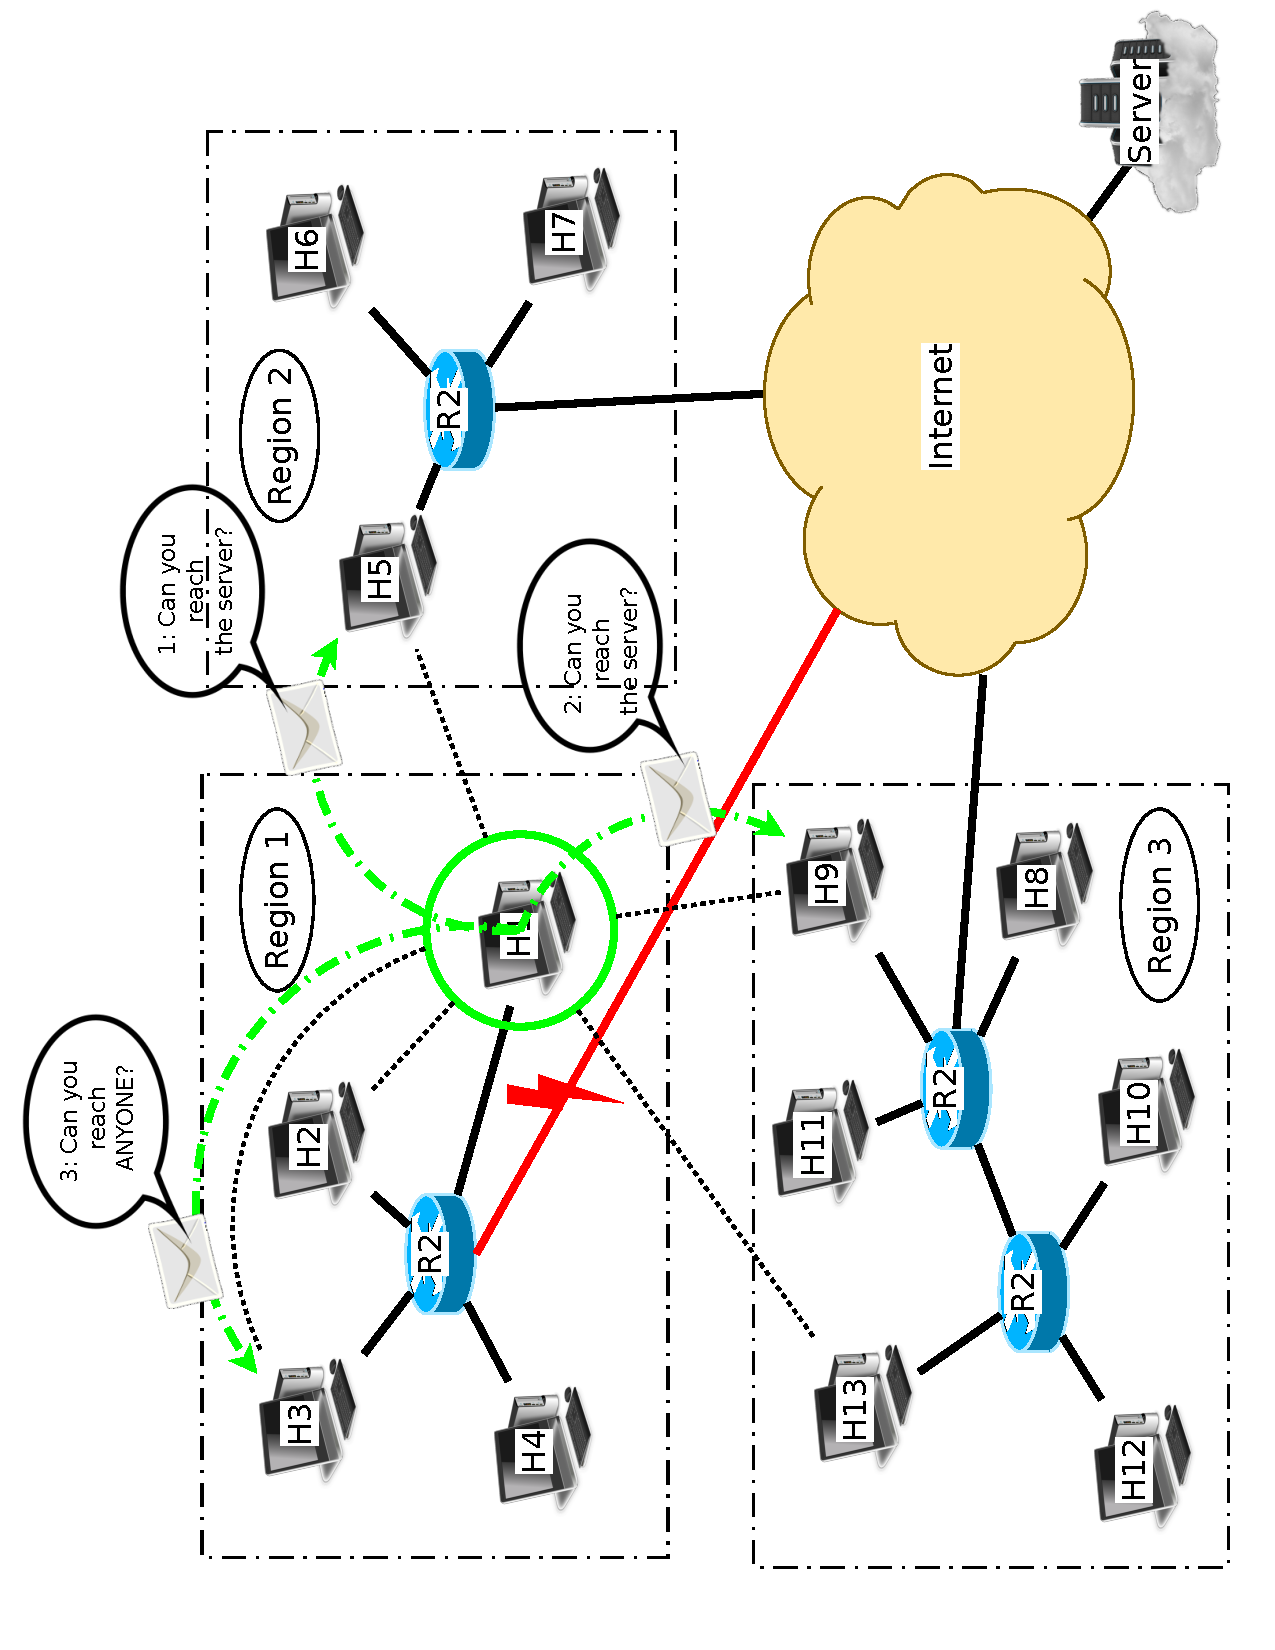
\includegraphics[height=\textwidth,angle=-90]{new_region_all}
\caption{The intuition of this heuristic is to avoid regions that have been previously attempted unsuccessfully.  We assume that no further attempts to contact such a region will succeed.}
\end{figure}
\end{column}

\end{columns}
\end{frame}


% % % % % % % % % % % % % % % % % % % % % % % % % % % % % % % % % % % % % % % % % %
\begin{frame}{New Angle Path Heuristic}
\begin{columns}

\begin{column}{.5\textwidth}
\begin{algorithm}[H]
\DontPrintSemicolon
\SetKwBlock{Begin}{begin}{end}
\SetAlgoLined
\SetAlgoLongEnd
\scriptsize
\Begin{
\tcc*[l]{For angle-dependent path heuristic algorithm.}
\lIf{$angle = \pi$ {\bf or} $angle = 0$} {$likelihood = 0$\;}
\lElseIf{$angle < \pi$} {$likelihood = \cos (angle - 0.25 \cdot \pi)$\;}
\lElseIf{$angle > \pi$} {$likelihood = \cos (2 \cdot ((2 \cdot \pi - angle) - 0.25 \cdot \pi)/3)$\;}
}
\caption{New Angle Path Heuristic Algorithm}
\small
\end{algorithm}
\end{column}
	
\begin{column}{.5\textwidth}
\begin{figure}
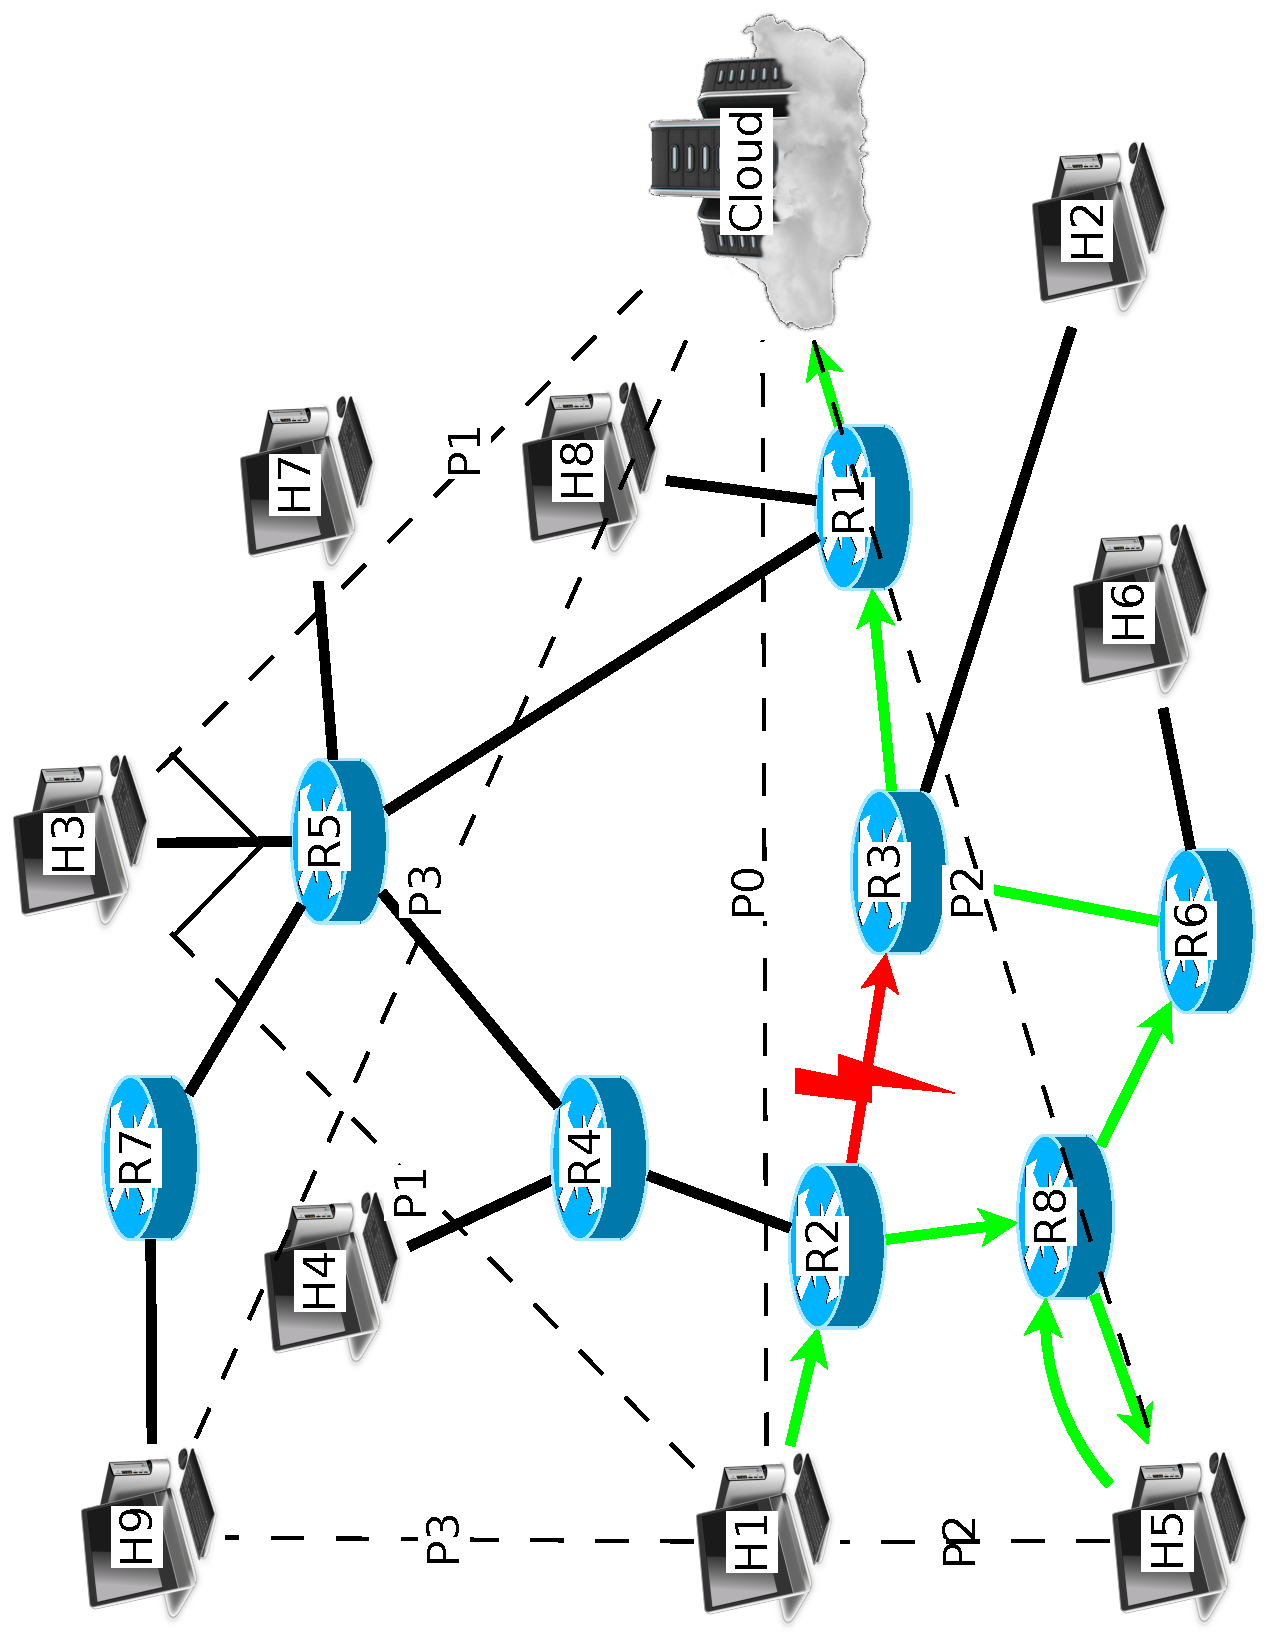
\includegraphics[height=\textwidth,angle=-90]{new_angle}
\caption{This heuristic attempts paths along new angles different from the ones previously attempted.}
\end{figure}
\end{column}

\end{columns}
\end{frame}

% % % % % % % % % % % % % % % % % % % % % % % % % % % % % % % % % % % % % % % % % %

\begin{frame}{Distance-Dependent Path Heuristic}
\begin{columns}
\begin{column}{.5\textwidth}
\begin{algorithm}[H]
\DontPrintSemicolon
\SetKwBlock{Begin}{begin}{end}
\SetAlgoLined
\SetAlgoLongEnd
\scriptsize
%\SetAlgoSkip{bigskip}
%\SetAlgoInsideSkip{medskip}
%$/*Initialization*/$\;
\Begin{
\tcc*[l]{For distance-dependent path heuristic algorithm.}
\lIf{$distance < minDistance$} {$likelihood = 0$\;}
\lElseIf{$minDistance < distance < mDistance$} {$likelihood = 0.4 \cdot (distance - minDistance)$\;}
\lElseIf{$mDistance < distance < maxDistance$} {$llikelihood = (distance - minDistance)$\;}
\lElseIf{$distance > maxDistance$} {$likelihood = 0.8 \cdot (distance - minDistance)$\;}
}
\caption{Distance-Dependent Path Heuristic Algorithms}
\small
\end{algorithm}
\end{column}
	
\begin{column}{.5\textwidth}
\begin{figure}
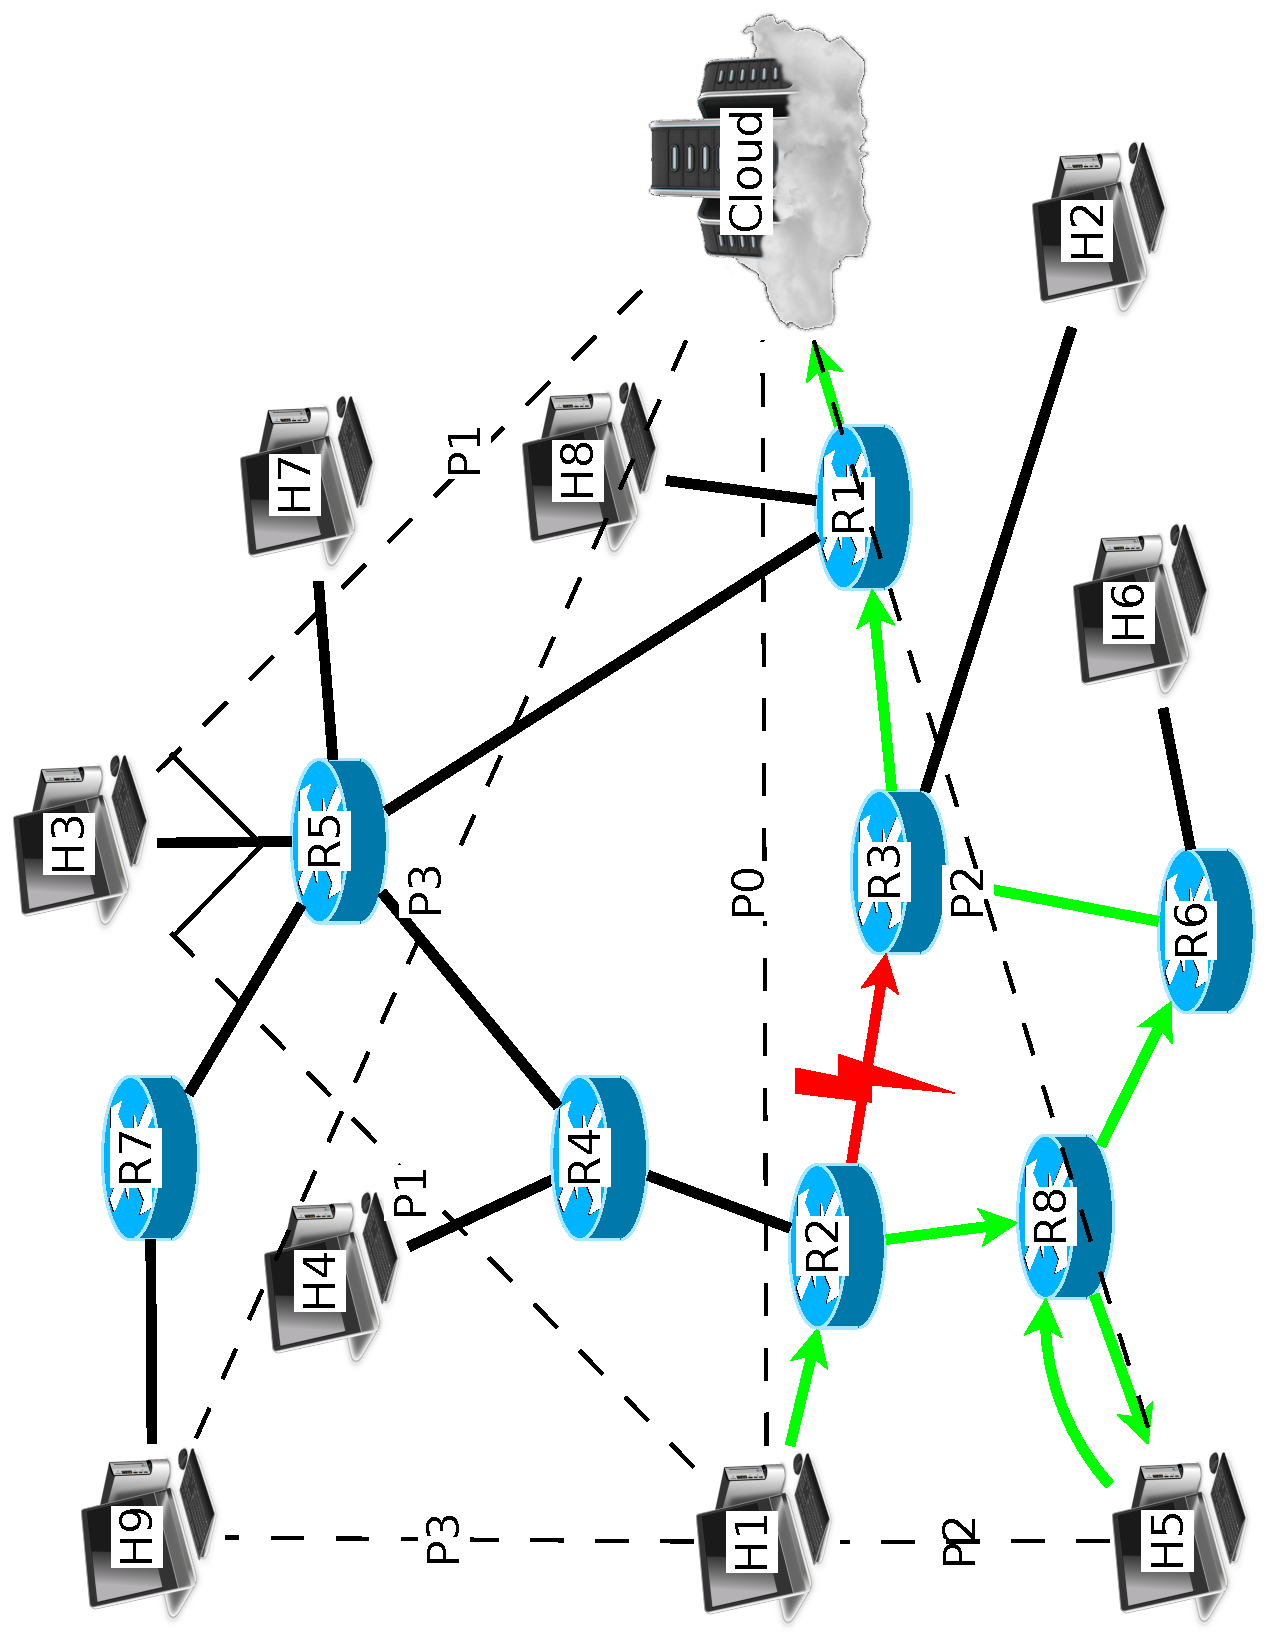
\includegraphics[height=\textwidth,angle=-90]{new_angle}
\caption{This heuristic attempts paths that use overlay nodes at an ideal distance from the sensor.  This ideal distance is chosen as a radius that reaches half-way to the server.}
\end{figure}
\end{column}

\end{columns}
\end{frame}

% % % % % % % % % % % % % % % % % % % % % % % % % % % % % % % % % % % % % % % % % %

\begin{frame}{Closest First Path Heuristic}
\begin{columns}
\begin{column}{.5\textwidth}
\begin{itemize}
	\item Failure along path to server or in local area
	\item Choose node that has the largest distance from the source
	\item Choose path avoiding as much of the direct path as possible
	\item Overlay node may use similar route to sensor
\end{itemize}
\end{column}
	
\begin{column}{.5\textwidth}
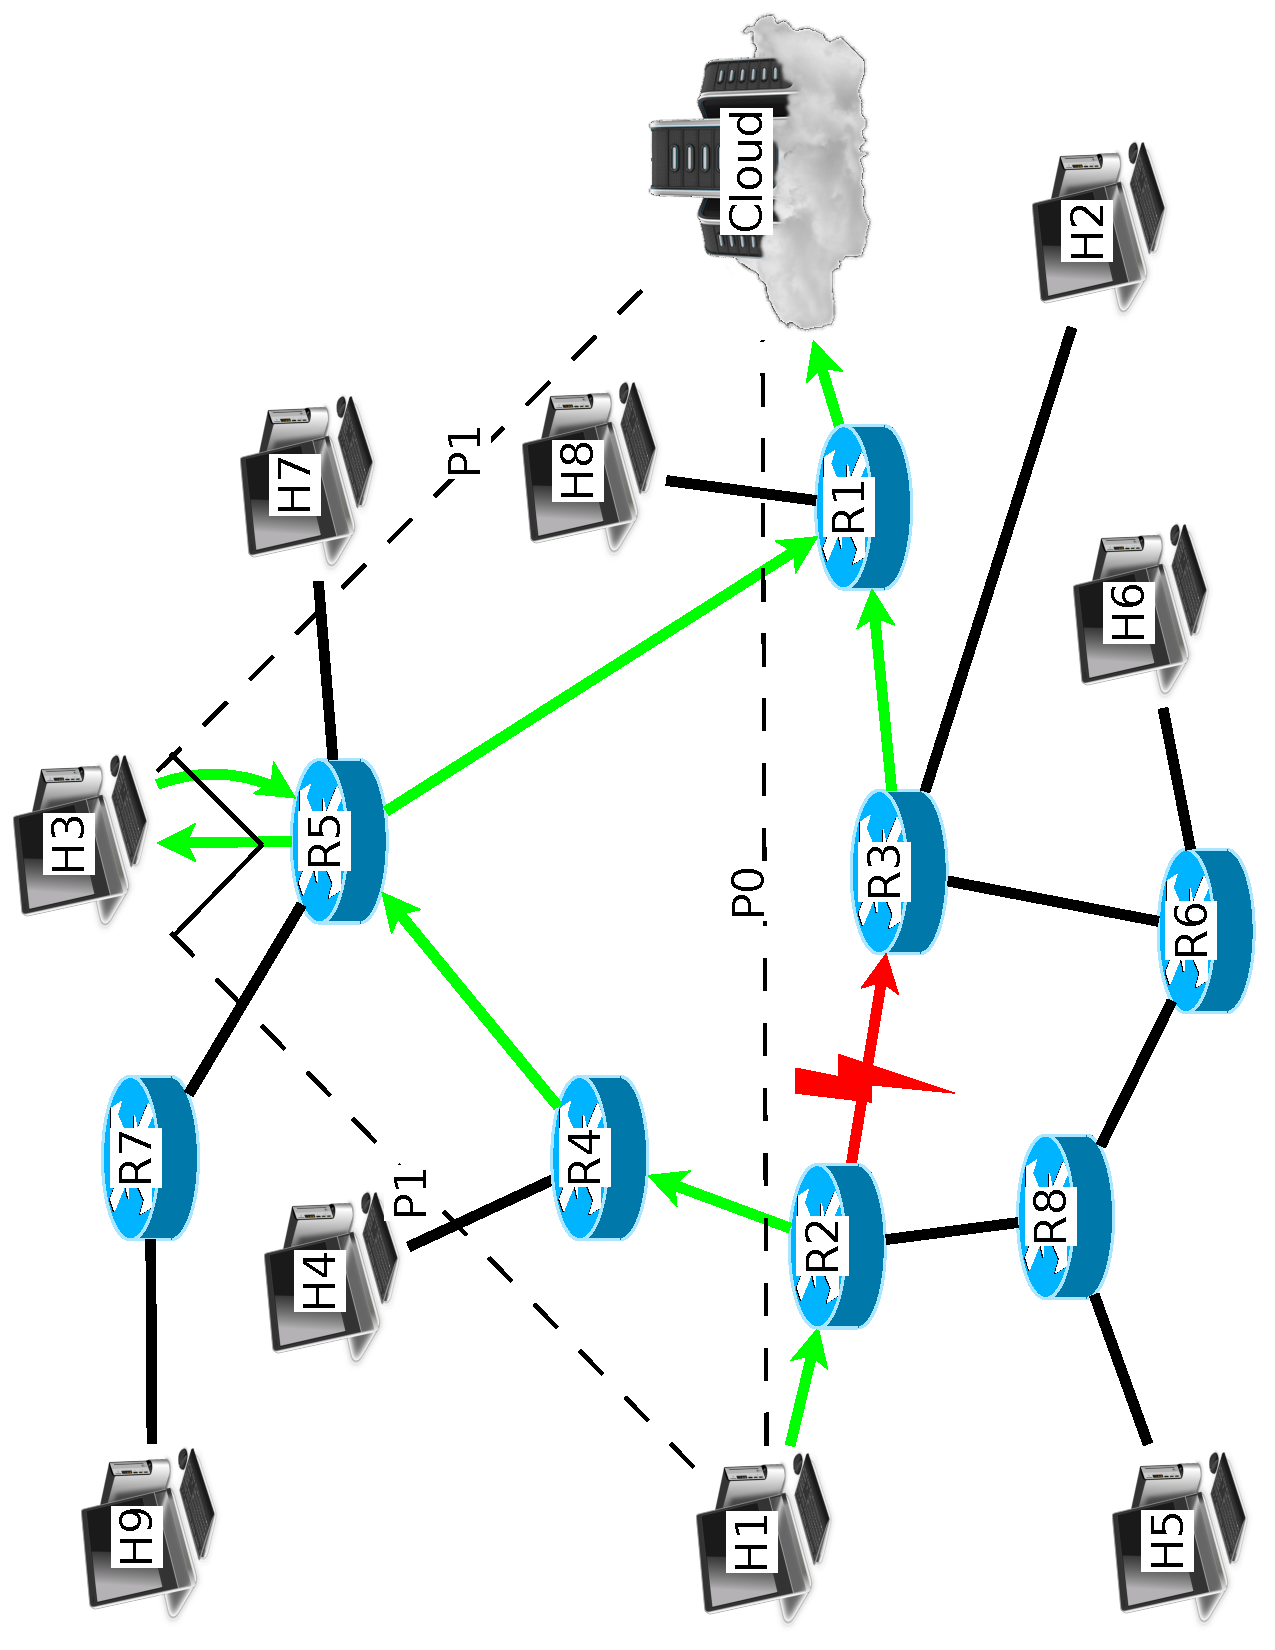
\includegraphics[height=\textwidth,angle=-90]{angular_path}
\end{column}

\end{columns}
\end{frame}

% % % % % % % % % % % % % % % % % % % % % % % % % % % % % % % % % % % % % % % % % %

\begin{frame}{Furthest First Path Heuristic}
\begin{columns}
\begin{column}{.5\textwidth}
\begin{itemize}
	\item Failure along path to server or in local area
	\item Choose node that has the largest distance from the source
	\item Choose path avoiding as much of the direct path as possible
	\item Overlay node may use similar route to sensor
\end{itemize}
\end{column}
	
\begin{column}{.5\textwidth}
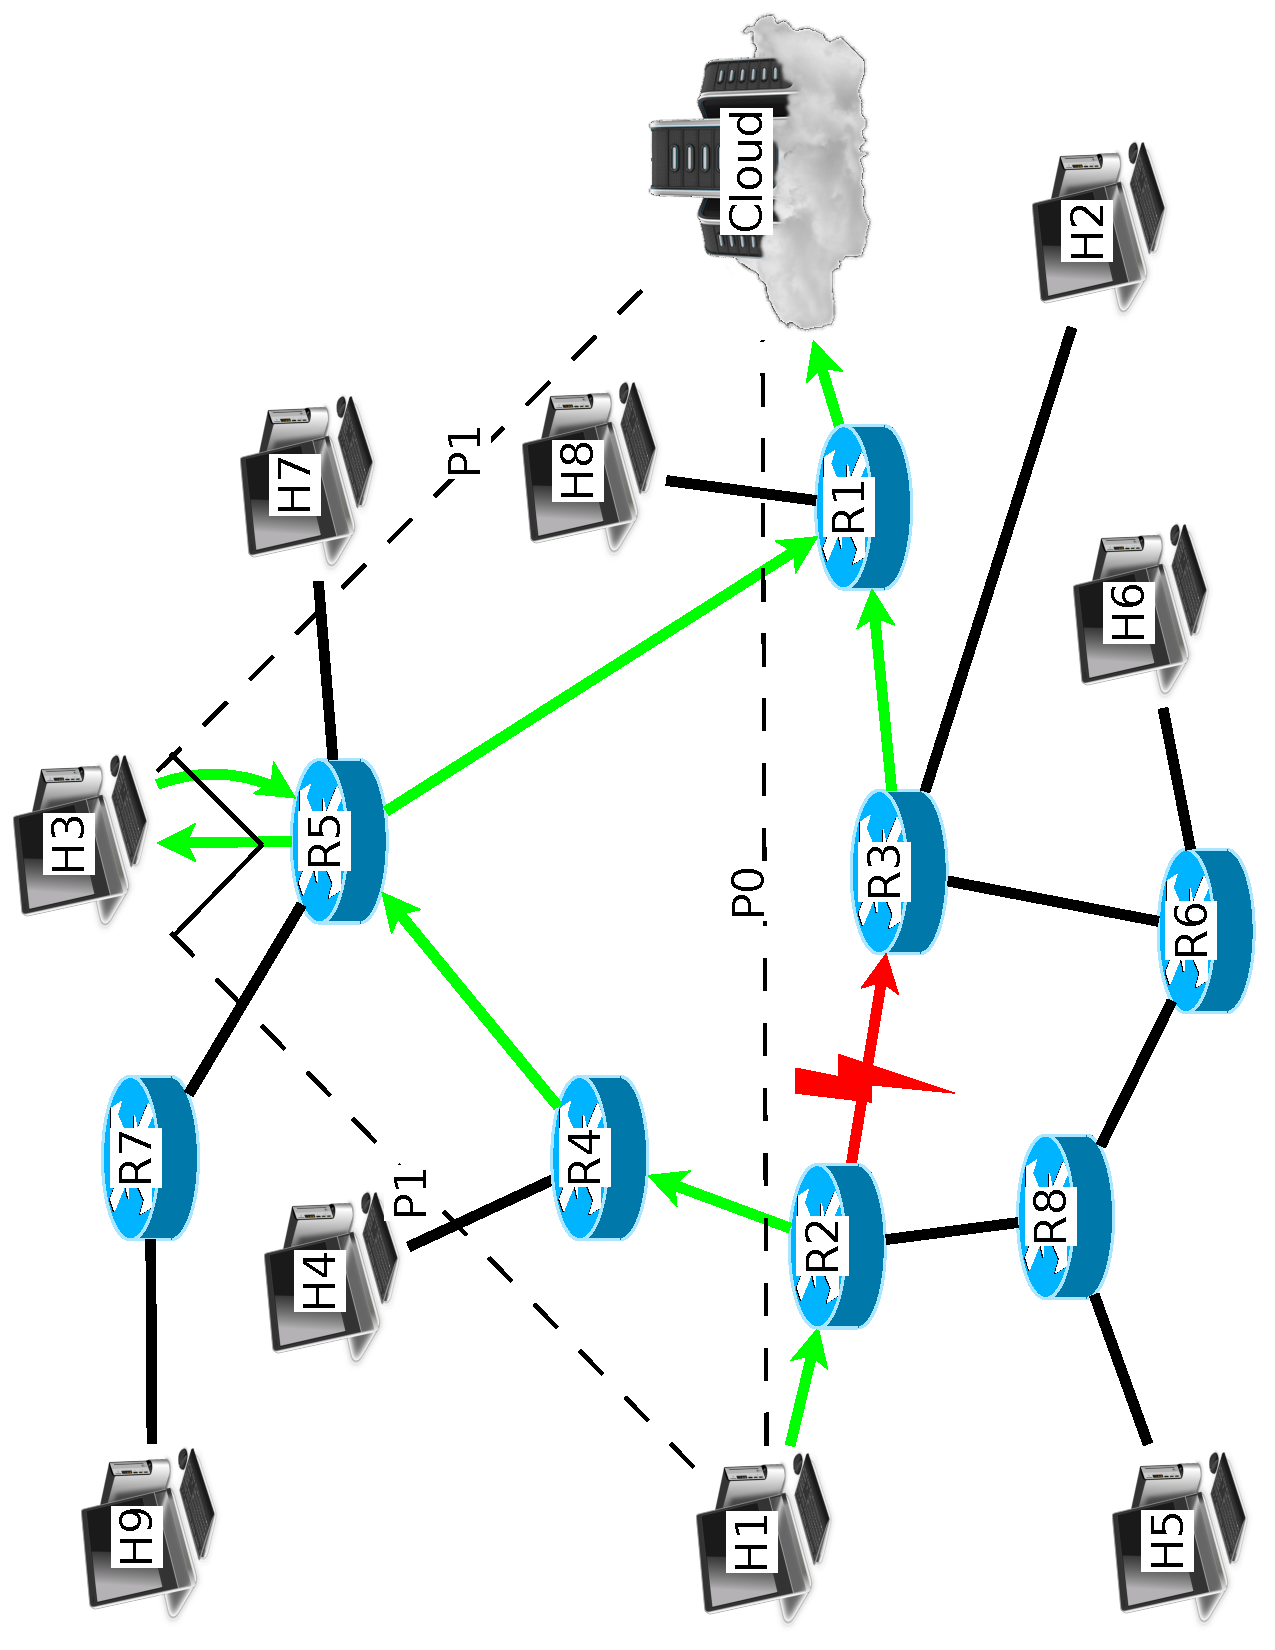
\includegraphics[height=\textwidth,angle=-90]{angular_path}
\end{column}

\end{columns}
\end{frame}


%
%\part{rest}
%
%\begin{frame}{Roadmap}
%	\tableofcontents
%\end{frame}
%
%\section{Location Service}
%
%\begin{frame}{Location Service}
%\begin{columns}
%\begin{column}{.5\textwidth}
%
%	\begin{itemize}
%		\item Nodes have GPS
%		\item But how to look up destination's location?
%		\item Maintain global information \uncover<2->{\alert{easily outdated/inefficient}}
%		\item<3-> Distribute load
%		\begin{itemize}
%			\item In , node updates \emph{location servers} (LS) throughout network
%			\item Divide network into hierarchical grid
%			\item LS's in 3 external grids at each level
%			\item Lookup distance $<$ square LS co-resides in
%		\end{itemize}
%		
%	\end{itemize}
%
%\end{column}
%
%\begin{column}{.5\textwidth}
%\uncover<3->{
%\begin{figure}
%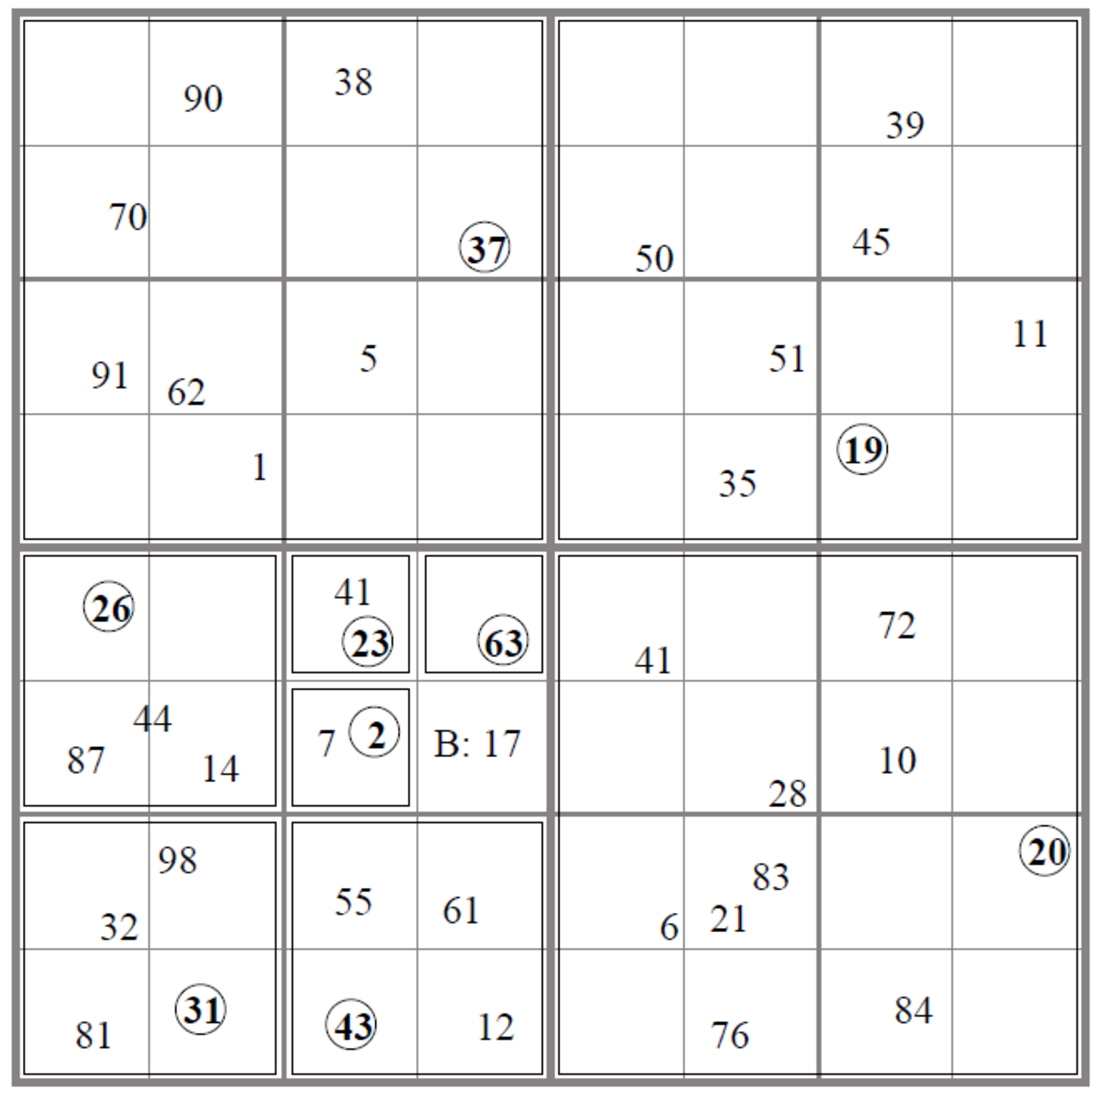
\includegraphics[width=\textwidth]{location_service}
%\caption{Hierarchical grid with 4 order-i squares in order-i+1 square.}
%\end{figure}}
%\end{column}
%\end{columns}
%\end{frame}
%

\end{document}
